\chapter{Metodologia badań}
\par W kontekście badań nad optymalizacją zespołów projektowych, niezwykle istotne jest zrozumienie oraz zastosowanie odpowiedniej metodologii. Metodologia ta bazuje na modelu optymalizacyjnym, który umożliwia analizę i dobór najbardziej efektywnego składu zespołu w oparciu o zdefiniowane kryteria i ograniczenia. 
\par Głównym celem modelu optymalizacyjnego omawianego w pracy jest minimalizacja całkowitego kosztu zatrudnienia pracowników przy jednoczesnym zapewnieniu, że zespół będzie dysponował niezbędnymi umiejętnościami do realizacji projektu. Osiągnięcie tego celu wymaga precyzyjnego określenia kryteriów wyboru członków zespołu oraz zdefiniowania ograniczeń, takich jak budżet, czas dostępny na realizację projektu oraz minimalny poziom umiejętności jaki zespół musi spełnić, żeby zrealizować projekt w danym czasie i z satysfakcjonującym efektem końcowym.
\par Metodologia badań opiera się również na analizie zbioru danych dotyczących pracowników, które obejmują między innymi ich umiejętności technologiczne, oczekiwane wynagrodzenie i dostępność czasową. Wykorzystanie tych danych pozwala na konstrukcję modelu matematycznego, który przez techniki optymalizacyjne i wykorzystanie narzędzi programistycznych umożliwia znalezienie optymalnego rozwiązania problemu dobierania odpowiednich pracowników do zespołów.
\par W dalszych częściach niniejszego rozdziału zostaną przedstawione detale modelu optymalizacyjnego, w tym jego funkcja celu, zmienne decyzyjne i ograniczenia. Opisane zostanie również, jak zbiór danych został wykorzystany do implementacji modelu oraz jakie kryteria zostały przyjęte do oceny efektywności różnych konfiguracji zespołu. Finalnie, omówione zostaną ograniczenia modelu, które wynikają zarówno z założeń teoretycznych, jak i praktycznych aspektów jego zastosowania w realnych warunkach zarządzania projektami w branży IT.


\section{Opis modelu optymalizacyjnego}
\par Model optymalizacyjny zaprezentowany w tej pracy ma na celu zoptymalizowanie składu zespołu programistów pracujących nad projektem IT, z uwzględnieniem ograniczeń budżetowych oraz czasowych. Bazując na metodach programowania liniowego, model pozwala na efektywne zarządzanie zasobami ludzkimi w celu maksymalizacji efektywności pracy przy jednoczesnym minimalizowaniu kosztów. Model ten używa oprogramowania PuLP, które jest biblioteką w języku Python przeznaczoną do rozwiązywania problemów optymalizacyjnych liniowych i całkowitoliczbowych.
\par W projekcie wykorzystany jest skrypt \verb|generator.py|, który odpowiada za generowanie losowego zbioru danych pracowników, używany do testowania i walidacji modelu optymalizacyjnego. 

\section{Proces budowy modelu optymalizacyjnego}
\par Budowa modelu optymalizacyjnego jest złożonym procesem, który wymaga precyzyjnego zrozumienia zarówno matematycznych, jak i praktycznych aspektów problemu. Taki proces obejmuje kilka kluczowych kroków, które zostaną omówione poniżej. Każdy z tych kroków jest kluczowy dla stworzeniu modelu, który nie tylko będzie działać, ale też spełni swoje zdanie w praktyce. Jak stwierdza Kerzner H. w swojej książce doskonałość (w kontekście optymalności zespołów) nie zostanie osiągnięta bez zmiany, a szybkość tej zmiany jest krytyczna dla osiągnięcia doskonałości \parencite{kerzner2003advanced}.
    \subsection{Definicja problemu}
    \par Pierwszym krokiem w budowie modelu LP jest jasne zdefiniowanie problemu, który ma zostać poddany optymalizacji. Kluczowe jest, aby na początku określić, co dokładnie chcemy osiągnąć za pomocą optymalizacji. Tezę te potwierdza książka Leach L. \parencite{leach2014critical}. W kontekście zespołów projektowych problem, a zarówno celem może być maksymalizacja efektywności zespołu, minimalizacja kosztów lub zbalansowanie obciążenia pracą. Definiowanie problemu może obejmować:
    \begin{description}
        \item[Określenie celów] - Co dokładnie ma nam dać optymalizacja? Trzeba jasno zdecydować, co jest głównym celem tego procesu; czy jest to minimalizacja kosztów, maksymalizacja produktywności pracowników czy zwiększenie przydziału pracy na pracownika. Według Katz'a i in. \parencite{katz1980system} Zdefiniowanie terminologii naturalnej dla danej dziedziny problemowej jest pierwszy etapem w konstrukcji modelu LP.
        \item[Identyfikacje ograniczeń] -  Jakie są główne ograniczenia wpływające na model? Co przede wszystkim ogranicza cel optymalizacji; może to być budżet, czas lub zasoby. Niezależnie od tego co to jest, określenie tego na początku procesu pozwala na sprawne przeprowadzenie optymalizacji.
    \end{description}

    \subsection{Zbieranie i analiza danych}
    \par Dane są kluczowym elementem każdej optymalizacji, a proces ich zbierania i przygotowania może mieć kluczowy wpływ na jej wynik. Jak stwierdzają Katz i in. \parencite{katz1980system} baza danych jest używana do przypisywanie wartości identyfikatorom, reprezentującym stałe abstrakcyjne w modelu. Do najważniejszych etapów w procesie przygotowywanie danych można zaliczyć:
    \begin{description}
        \item[Zbieranie danych] - Gromadzenie wszystkich niezbędnych informacji, które później będą użyte w modelu optymalizacyjnym. W kontekście zespołu projektowego mogą to być dane ewaluacyjne pracowników, ich oczekiwane zarobki, ich efektywność w danych dziedzinach i ogólna produktywność.
        \item[Czyszczenie danych] - Przygotowanie danych do dalszej pracy wymaga sprawdzenia czy dane nie zawierają błędów, duplikatów lub ewentualnych braków. W przypadkach gdy takowe się pojawią, należy je odpowiednio przerobić i upewnić się, że całość danych jest spójna i dokładna.
        \item[Przekształcenie danych] - Po uporządkowaniu, dane należy odpowiednio sformatować, żeby model mógł z nich skorzystać. Dokładne implementacja zależy od modelu, niemniej jednak trzeba zadbać, o dobry format danych wejściowych w celu uniknięcia błędów.
    \end{description}

    \subsection{Wybór technik i narzędzi optymalizacyjnych}
    \par Odpowiednie dobranie techniki do problemu, może być kluczowe dla skuteczności optymalizacji oraz czasu jaki musi zostać na to poświęcony. Pod rozważanie można wziąć różne techniki takie jak programowanie liniowe, heurystyki oraz metaheurystyki. Do tego należy zdecydować jak model zostanie zaimplementowany. Wybór jest niezwykle szeroki i między innymi można wybrać spośród języka programowania Python, MATLAB czy środowiska R, ale też można korzystać z narzędzi takich jak Microsoft Excel.

    \subsection{Budowa modelu matematycznego}
    \par Na proces budowy modelu matematycznego składają się wszystkie poprzednie kroki, ale tylko ich uprzednie wykonanie pozwala na udaną budowę. Abstrakcyjny model matematyczne jest, według Katz'a i in., tworzony poprzez wymienienie dowolnej liczby ograniczeń i dokładnie jednej funkcji celu \parencite{katz1980system}. Ten proces można zawęzić do:
    \begin{description}
        \item[Definiowanie zmiennych decyzyjnych] - Polega przede wszystkim na ustaleniu jakie czynniki, będą decydowały o statusie optymalizacji. Na przykład, jeśli optymalizacja polega na znalezieniu jak najbardziej wydajnych pracowników, zmienna decyzyjna będzie określać czy dany pracownik jest odpowiednio wydajny, w stosunku do reszty. Analogicznie, przy optymalizacji zasobów, będzie określać czy dane sposób na wytworzenie konkretnej ilości produktu, jest optymalny. Zmienna decyzyjna może przyjmować wartość 1 - dla optymalnego wyboru, lub 0 - dla wyborów nieoptymalnych.
        \item[Formułowanie funkcji celu] - Kolejnym etapem jest sformułowanie funkcji celu. Funkcja ta jest wyrażeniem matematycznym, które opisuje, co chcemy optymalizować. Według Winstona \parencite{winston2004operations}, funkcja celu w modelu programowania liniowego wskazuje na maksymalizacje (zysków lub wydajności) lub minimalizacje (kosztów). W przypadku optymalizacji zespołów projektowych funkcja celu może uwzględniać takie czynniki jak całkowity koszt zatrudnienia, poziom kompetencji zespołu czy czas realizacji projektów.
        \item[Ustalenie ograniczeń] - Każdy model optymalizacyjny musi uwzględniać ograniczenia, które odzwierciedlają rzeczywiste zasoby i ograniczenia problemu. Bazaraa i in. \parencite{bazaraa2010} podkreślają, że identyfikacja i precyzyjne sformułowanie ograniczeń jest kluczowym elementem procesu modelowania. Mogą to być ograniczenia dotyczące dostępności pracowników, budżetu, wymaganych umiejętności oraz terminów projektowych. Formułowanie tych ograniczeń w postaci równań lub nierówności jest niezbędne do uzyskania realistycznych i praktycznych wyników.
    \end{description}

    \subsection{Implementacja modelu w wybranym środowisku}
    \par Następnym krokiem jest implementacja modelu w praktyce. Vanderbei \parencite{vanderbei2001} podkreśla, że wdrożenie modelu wymaga użycia specjalistycznych narzędzi do programowania liniowego. Implementacja powinna być monitorowana i aktualizowana w miarę potrzeb, aby zapewnić ciągłą optymalizację procesu. Regularne aktualizacje i monitorowanie są kluczowe dla adaptacji modelu do zmieniających się warunków i wymagań projektowych.
    
    \subsection{Walidacja i testowanie modelu}
    \par Po stworzeniu modelu należy go zweryfikować i przetestować, aby upewnić się, że poprawnie odzwierciedla rzeczywistość i dostarcza praktyczne rozwiązania. Walidacja może obejmować testowanie modelu na różnych scenariuszach.

    \subsection{Analiza wyników i interpretacja}
    \par Po przeprowadzonej optymalizacji należy poświęcić czas na analizę wyników i wyciągnięcie z niej wniosków. Taka analiza może dostarczyć wartościowych informacji na temat przeprowadzonej optymalizacji. Ważnym jest zrozumienie jakie decyzje należy podjąć i jak one wpłyną na rzeczywiste operacje. Analiza może obejmować prostą analizę statystyczną, analizę wrażliwości i ocenę ryzyka. Dodatkowo, można przeprowadzić podobne analizy na danych sprzed optymalizacji i porównać wyniki przed i po.


\section{Przedstawienie zbioru danych}
\par Zbiór danych, wykorzystany w niniejszym modelu optymalizacyjnym, jest generowany programowo za pomocą skryptu \verb|generator.py|. Celowo zastosowano mechanizm generacji syntetycznych danych w celu unifikacji i kontrolowania warunków eksperymentu, co umożliwia precyzyjną analizę działania modelu optymalizacyjnego pod różnymi aspektami. Generowane dane odzwierciedlają potencjalne warunki rynkowe, w których działają specjaliści IT, pozwalając na symulację różnych scenariuszy zatrudnienia bez konieczności uzyskania dostępu do rzeczywistych danych osobowych. 
\par Dla urzeczywistnienia danych zastosowano rozkład normalny, a implementacja używa bibliotek \verb|NumPy| - dla metod matematycznych, \verb|Pandas| - dla łatwiejszej pracy z arkuszami \verb|.csv| oraz \verb|Names| - dla lepszej czytelności generowanych danych poprzez dodanie realistycznych imion dla generowanych pracowników. Biblioteka NumPy jest potężnym narzędziem stosowanym w wielu dziedzinach jak wskazują autorzy artykułu \parencite{harris2020array} "\textit{Odgrywa kluczową rolę w analizie danych badawczych w dziedzinach tak różnorodnych jak fizyka, chemia, astronomia, nauki o Ziemi, biologia, psychologia, nauki o materiałach, inżynieria, finanse i ekonomia.}".
\par Atrybuty generowane dla każdego z pracowników to:
\begin{description}
    \item[Imię i nazwisko] - dla lepszej czytelności danych
    \item[Umiejętności technologiczne] - umiejętności we framework’u Angular, umiejętności w języku programowania Java, umiejętności w design’ie UI/UX (Interfejs użytkownika / doświadczenia użytkownika), umiejętności w języku SQL i bazach danych oraz znajomość języka angielskiego. Umiejętności generowane są z rozkładu normalnego, o średniej = 0.4 i odchyleniu standardowym = 0.5. Zastosowanie metody \verb|np.clip()| zapewnia że generowane wartości będą mieścić się w przedziale $[0, 1]$. W rzeczywistym scenariuszu, takie statystyki mogłyby być pozyskane poprzez przeprowadzanie cyklicznych testów kompetencji pracowników z każdej z dziedzin, a ich wynik odpowiednio dostosowany do skali $[0, 1]$.
    \item[Suma umiejętności\label{itm:suma_umiejetnosci}] - jest wykorzystywana do realistycznego określenia stawki godzinowej jaką pracownik o danych umiejętnościach mógłby oczekiwać. 
    \item[Wynagrodzenie] - częściowo uzależnione od poziomu sumy umiejętności. Pracownikom znajdującym się powyżej trzeciego kwantyla sumy umiejętności zostanie przypisane wyższe wynagrodzenie z przedziału [70, 99], a tym znajdującym się poniżej zostanie przypisane wynagrodzenie z przedziału [30, 69]. Takie podejście pozwala na rzeczywiste zróżnicowanie wynagrodzenia pracownika zależnie od jego kwalifikacji co odzwierciedla warunki rynkowe, niezbędne dla zapewnienia trafności modelu oraz użyteczności programu.
\end{description}
\par Po wygenerowaniu, dane są eksportowane do pliku \verb|.csv| do wglądu i analizy oraz do późniejszego zastosowania w modelu optymalizacyjnym. Struktura danych jest ściśle związana z procesem tworzenia modelu oraz pozwala na wielokrotne testowanie modelu w oparciu o różnorodne dane. Tak generowany zbiór danych w rzeczywistości mógłby być zastąpiony, po odpowiednim opracowaniu danych, faktycznymi danymi rynkowymi w celu przeprowadzenia faktycznej analizy w rzeczywistym scenariuszu. Struktura danych w pliku z wygenerowanymi pracownikami \verb|.csv| wygląda następująco:
\begin{figure}[H]
    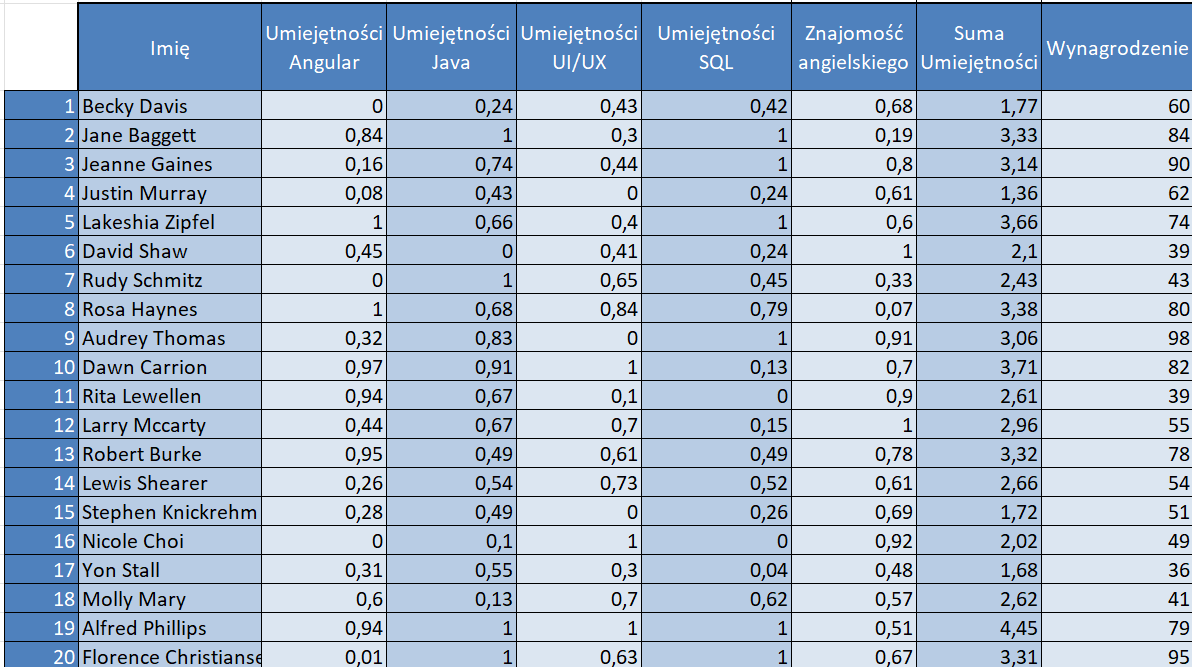
\includegraphics[width=\linewidth]{chapters/Images/pracownicy_csv.png}
    \cprotect\caption{Struktura danych pracowników w pliku \verb|.csv| po wygenerowaniu\\ Źródło:\textit{ opracowanie własne}}
\end{figure}

\par Tak utworzony zbiór danych stanowi podstawę do analizy możliwości modelu optymalizacyjnego przy różnych warunkach i ograniczeniach w kontekście zarządzania zespołami projektowymi w branży IT. Analiza danych umożliwi wykrycie istotnych wzorców i trendów, które bezpośrednio wpłyną na efektywność i skuteczność optymalnego zespołu projektowego.



\section{Omówienie kodu generatora danych}\label{sec:kod_generator}
\par Kod przedstawiony na grafice pełni rolę generatora danych dla pracowników w kontekście projektu IT. Przede wszystkim, generuje on dane dotyczące umiejętności technicznych i wynagrodzenia pracowników. Poniżej znajduje się szczegółowe omówienie każdej sekcji kodu z uwzględnieniem numeracji linii.

\lstinputlisting[language=Python, caption=Kod źródłowy generatora danych\\ Źródło:\textit{ opracowanie własne}]{generator.py}

\begin{description}
    \item[Linie 1-3] - Na początku skryptu importowane są trzy kluczowe biblioteki: \verb|numpy| (alias \verb|np|), \verb|pandas| (alias \verb|pd|) oraz \verb|names|. Biblioteka numpy jest używana do operacji matematycznych i generowania losowych danych, pandas do tworzenia i manipulacji strukturami danych, takimi jak DataFrame, a names do generowania losowych imion pracowników. 
    
    \item[Linie 5-8] Następnie, do linii 8 użytkownikowi wyświetlane są zapytania o wartości kluczowych zmiennych: \verb|liczba_pracownikow, srednia_umiejetnosci, odchylenie_standardowe| oraz \verb|nazwa_pliku_csv|. Od pierwszych trzech zależy finalny wygląd wygenerowanych danych, czwarta określa nazwę pliku do zapisu wyników.
    
    \item[Linie 10-12] W tych liniach tworzony jest słownik \verb |dane_pracownikow|, który początkowo zawiera jedynie losowo wygenerowane imiona pracowników. Imiona są generowane przy użyciu funkcji \verb |names.get_full_name()| w pętli dla wszystkich pracowników.
    
    \item[Linie 14-18] - Następnym krokiem jest zdefiniowanie listy umiejętności (\verb|umiejetnosci|), które będą przypisane do pracowników: \verb|Umiejetnosci Angular, Umiejetnosci Java,| \verb|Umiejetnosci UI/UX, Umiejetnosci SQL| i \verb|Znajomosc angielskiego|. Dla każdej umiejętności w liście, generowane są losowe wartości przy użyciu rozkładu normalnego z określoną średnią i odchyleniem standardowym. Wartości te są zaokrąglane do dwóch miejsc po przecinku i ograniczane do przedziału $[0, 1]$ za pomocą metody \verb|np.clip()|. Po wygenerowaniu danych, lista pracowników jest przekształcona w \verb|DataFrame|.
    
    \item[Linie 19-21] - W tych liniach obliczana jest wartość sumy umiejętności dla każdego pracownika oraz 75. percentyl, na którego podstawie ustalane jest wynagrodzenie. Jeśli suma umiejętności pracownika jest większa od kwantyla sumy umiejętności pracowników, dostaje on wynagrodzenie losowane z przedziału $[70, 99]$. W przypadku wartości niższej wynagrodzenie losowane jest z przedziału $[30, 69]$.
    \item[Linie 23-25] - Na koniec wykonywania skrypt wyświetla pierwsze wiersze pliku z danymi pracowników i wyświetla nazwę pod która plik został zapisany.
\end{description}

\section{Kryteria i ograniczenia modelu}\label{sec:ograniczenia_modelu}
\par Kryteria, które definiują budowę oraz proces tworzenia modelu optymalizacyjnego są ściśle związane z osiągnięciem najwyższej możliwie efektywności zespołu projektowego przy minimalizowaniu kosztów utrzymania takiego zespołu. Te kryteria są odwzorowane pod postaciami funkcji celu, ograniczeń oraz zmiennych decyzyjnych. Funkcja celu dąży do minimalizacji kosztów utrzymania zespołu projektowego przy jednoczesnym zapewnieniu jak największego poziomu umiejętności z każdej kategorii dla zapewnienia jak najwyższej jakości wykonywanego projektu przy określonym budżecie przeznaczonym na pracę.
\par Model przestrzega szeregu ograniczeń, które determinują finalny skład zespołu projektowego. Dla zapewnienia realistycznego scenariuszu zostały przyjęte dwa główne ograniczenia: ograniczenie budżetowe oraz ograniczenie minimalnych umiejętności zespołu. 

\begin{description}
    \item[Ograniczenie minimalnych umiejętności zespołu] - istnieje w celu określenia złożoności projektu. W obecnej branży IT, poziom zaawansowania i stopień trudności wykonania projektu jest wielce zróżnicowany i jego dokładne określenie, może znacząco ułatwić przebieg prac. Odpowiednie dobranie członków zespołu, który ma nad nim pracować, może znacząco ułatwić ten proces. Ograniczenie można przedstawić następującym wzorem:
    \[
        \sum_{i \in \mathcal{P}}^{n} \sum_{Skill \in \mathcal{U}}^{m} i_{Skill} \leq req
    \]
    gdzie:
    \begin{itemize}
        \item $n$ to liczba wszystkich pracowników zawartych w pliku \verb|pracownicy.csv|
        \item $\mathcal{P}$ to zbiór wszystkich pracowników w pliku \verb|pracownicy.csv|
        \item $m$ to liczba umiejętności wyróżnionych w tabeli w pliku \verb|pracownicy.csv|
        \item $\mathcal{U}$ to zbiór wszystkich umiejętności zawartych w tabeli w pliku \verb|pracownicy.csv|
        \item $Skill$ to wartość umiejętności $Skill$ dla pracownika $i$ z zakresu $[0,1]$
        \item $i_{Skill}$ to poziom umiejętności $Skill$ dla pracownika $i$
        \item $req$ to minimalny wymagany poziom umiejętności pracownika w zespole
    \end{itemize}
    
    \item[Ograniczenie budżetowe] - zobowiązuje model do przestrzegania ustalonego budżetu na zespół projektowy. Taki budżet może być określony przez na przykład klienta zlecającego projekt firmie IT lub wewnętrznie przez menadżera zespołu w przypadku gdy zlecenie obejmuje więcej usług niż tylko projekt IT. Budżet jest implementowany poprzez typ integer w celu zapewnienia, że budżet będzie liczbą całkowitą.
    Sprawdzenie czy model spełnia to ograniczenia wiąże się z obliczeniem czy wynagrodzenie godzinowe wybranych pracowników pomnożone przez liczbę godzin na projekt, jest mniejsze od zadanego budżetu. Ograniczenie to można opisać wzorem:
    \[
    \sum_{i \in \mathcal{P}}^{n} (x_i \cdot w_i \cdot h) \leq B
    \]
    
    gdzie:
    \begin{itemize}
        \item $\mathcal{P}$ to zbiór wszystkich pracowników w zbiorze danych
        \item $x_i$ to zmienna decyzyjna określająca, czy pracownik $i$ jest wybrany do zespołu (1 jeśli wybrany, 0 w przeciwnym razie)
        \item $K_i$ to wynagrodzenie godzinowe pracownika $i$
        \item $h$ to liczba godzin pracy nad projektem
        \item $B$ to maksymalny dostępny budżet
        \item $n$ to liczba pracowników w pliku \verb|pracownicy.csv|
    \end{itemize}
\end{description}

\par Oprócz ograniczeń wymaganych do funkcjonalności modelu, istnieją też ograniczenia które nie były dotąd poruszane w jego kontekście i mogą być niejawne, a możliwy jest ich znaczący wpływ na efektywność i skuteczność modelu.

\par Pierwszym z nich jest dostępność i format danych. Wyniki modelu są ściśle związane i zależne od danych wejściowych. Jakość, ilość oraz kompletność danych ma bezpośredni wpływ na końcowy wynik optymalizacji. Jeśli dane są niekompletne, nieprecyzyjne lub zniekształcone model może wygenerować suboptymalne, a w skrajnych przypadkach błędne wyniki. Dlatego też ważnym aspektem przy przeprowadzaniu takiej optymalizacji jest upewnienie się, że dane wejściowe są dokładne i kompletne.

\par Drugim jest mała elastyczność na zmieniające się czynniki i wymagania. Ten model został zaprojektowany dla stałych parametrów i ograniczeń i może nie spełniać swojej funkcji, gdy któraś z tych rzeczy ulegnie zmianie. Na przykład, jeśli budżet lub czas na wykonanie projektu ulegnie zmianie w trakcie trwania projektu, model może wymagać ponownej kalibracji lub nawet całkowitej przebudowy. W praktyce oznacza to, że model powinien być stosowany w przede wszystkim stabilnym środowisku, w którym parametry projektu są dobrze znane i nie są podatne na częste zmiany. W przeciwnym razie, każda zmiana może wymagać modyfikacji modelu, co może prowadzić do zwiększenia kosztów i utraty cennego czasu. 

\par Ostatnim jest preferowanie najniższego kosztu nad jakością zespołu. Priorytetem w obecnej implementacji modelu jest całkowity koszt zespołu ponad jego jakością. Oznacza to, że model będzie tworzył zespoły złożone z mniej wykwalifikowanych pracowników w celu utrzymania jak najniższych kosztów. Mimo tego, że model stara się utrzymać dany poziom umiejętności w zespole, jego głównym celem jest minimalizacja kosztów. W sytuacjach, gdzie jakość jest kluczowym czynnikiem, zastosowanie tego modelu może nie być najlepszym wyborem. W takich sytuacjach, należałoby zaimplementować model w taki sposób, żeby dążył do jak najwyższego poziomu umiejętności w zespole, a sprawa budżetu była drugorzędna.

\par Zrozumienie tych dodatkowych ograniczeń, pozwala na lepsze zrozumienie w jakich sytuacjach i kontekstach model optymalizacyjny najlepiej spełni swoje zadanie. Dodatkowo można dzięki temu zrozumieć i przewidzieć jakie wyzwania może napotkać model w trakcie optymalizacji. Dzięki szerszemu zrozumieniu, można być lepiej przygotowanym do pracy z tym modelem i skuteczniej dobierać dla niego zadania.

